\chapter{L'algoritmo ACS}%
\label{cha:L'algoritmo ACS}
In capitolo capitolo viene descritto il funzionamento dell'algoritmo
Alternating Criteria Search: viene definita la struttura dei sub-MIP e
vengono descritti i passi che permettono all'algoritmo di ottenere una
soluzione ammissibile per un problema MIP generico.

\section{Struttura dei problemi ausiliari}%
\label{sec:Struttura dei problemi ausiliari}
Prendiamo in considerazione il seguente MIP:
\begin{equation}
    \begin{cases}
        \min c^tx\\
        Ax = b\\
        l \leq x \leq u\\
        x_i \in \Z & \forall i\in I
    \end{cases}
\end{equation}
dove $c\in \R^m$, $A\in \R^{m\times n}$, $b\in \R^m$, $I\subseteq \{ 1, \ldots, n\}$
è l'insieme contenente gli indici delle variabili intere, $x$ è il vettore
delle variabili, infine $l\in \overline \R^n$ e $u\in \overline \R^n$ sono i
limiti imposti alle variabili e $\overline \R = \R \cup \{-\infty, +\infty\}$.

\subsection{FMIP}%
\label{sub:FMIP}
Il modello di FMIP è il seguente:
\begin{equation} \label{eq:FMIP}
    \begin{cases}
        \min \sum\limits_{i=0}^{m-1} \Delta_i^+ + \Delta_i^- \\
        Ax + I_m \Delta^+ - I_m \Delta^- = b \\
        x_i = \hat x_i & \forall i \in F \\
        l \leq x \leq u\\
        x_i \in \Z & \forall i \in I\\
        \Delta^+ \leq 0,\quad \Delta^- \leq 0
    \end{cases}
\end{equation}
dove $I_m\in \R^{m\times m}$ è la matrice identità e $\Delta^+$, $\Delta^-$
sono due vettori di variabili continue aventi dimensione $m$ in accordo
con il numero di vincoli del problema.
FMIP è ottenuto da MIP andando a modificare la funzione obiettivo e
aggiungendo variabili $\Delta^+_i,\,\Delta^-_i$ chiamate \emph{slack}.
Dalla \ref{eq:FMIP} notiamo che una soluzione ammissibile per FMIP
è ammissibile anche per il MIP se e solo se le variabili slack sommano
a zero.
FMIP non viene risolto direttamente ma vengono fissate un sottoinsieme
$F\subseteq I$ delle variabili intere a devi valori 
presi dal vettore di input $[\hat x,\,\, \Delta^+,\,\, \Delta^-]$.
La presenza delle variabili di slack permette di utilizzare un vettore $\hat x$ 
che non è necessariamente una soluzione ammissibile, l'unica restrizione 
è che siano rispettati i vincoli di interezza e i limiti delle variabili.
In altre parole si deve avere che $l \leq \hat x \leq u$ e $\hat x_i \in \Z,\, \forall i\in I$.

Minimizzare la somma delle slack permette di migliorare il grado di ammissibilità
della soluzione mentre il fissaggio delle variabili consente di ridurre la
complessità del problema.

% TODO: Aggiungo il caso in cui Ax<=b e Ax >= b?

\subsection{OMIP}%
\label{sub:OMIP}
Il secondo problema ausiliario ha come obiettivo quello di migliorare 
il vettore parzialmente ammissibile $[\hat x,\,\, \hat \Delta^+,\,\, \hat \Delta^-]$
che riceve in input.
Il suo modello si ottiene partendo dal MIP e aggiungendo ad ogni vincolo le 
variabili slack:
\begin{equation}
    \begin{cases}
        \min c^tx\\
        Ax + I_m \Delta^+ - I_m \Delta^- = b \\
        \sum\limits_{i=0}^{m-1} \Delta^+_i + \Delta^-_i \leq \sum\limits_{i=0}^{m-1} \hat \Delta^+_i + \hat \Delta^-_i\\
        x_i = \hat x_i & \forall i \in F \\
        l \leq x \leq u\\
        x_i \in \Z & \forall i\in I
    \end{cases}.
\end{equation}
In maniera analoga a FMIP, anche in OMIP vengono fissate alcune delle
variabili intere per ridurre la complessità del problema.
L'insieme $F$ non deve essere necessariamente lo stesso di \ref{eq:FMIP}.
Infine, per assicurare che la soluzione ottima di OMIP rimanga, al caso
peggiore, tanto inammissibile quanto il vettore di input $\hat x$, viene
aggiunto il vincolo 
$\sum_i \Delta^+_i + \Delta^-_i \leq \sum_i \hat \Delta^+_i + \hat \Delta^-_i$
che limita il valore della
somma delle variabili slack.

\section{Il processo risolutivo}%
\label{sec:Il processo risolutivo}
L'ACS inizia generando una soluzione di partenza intera $\hat x$, successivamente:
\begin{enumerate}
    \item Vengono fissate alcune variabili intere a $x_i = \hat x_i$ in FMIP.
    \item FMIP viene risolto, la sua soluzione è 
        $[\hat x,\,\, \Delta^+,\,\, \Delta^-]$.
    \item Vengono fissate alcune variabili intere a $x_i = \hat x_i$ in OMIP.
    \item OMIP viene risolto, la sua soluzione è 
        $[\hat x,\,\, \Delta^+,\,\, \Delta^-]$.
\end{enumerate}
Questi quattro passi vengono ripetuti iterativamente finché l'algoritmo non
converge ad una soluzione ammissibile, ovvero finché la somma delle variabili
slack è maggiore strettamente di zero.

\begin{figure}[ht!]
\begin{center}
    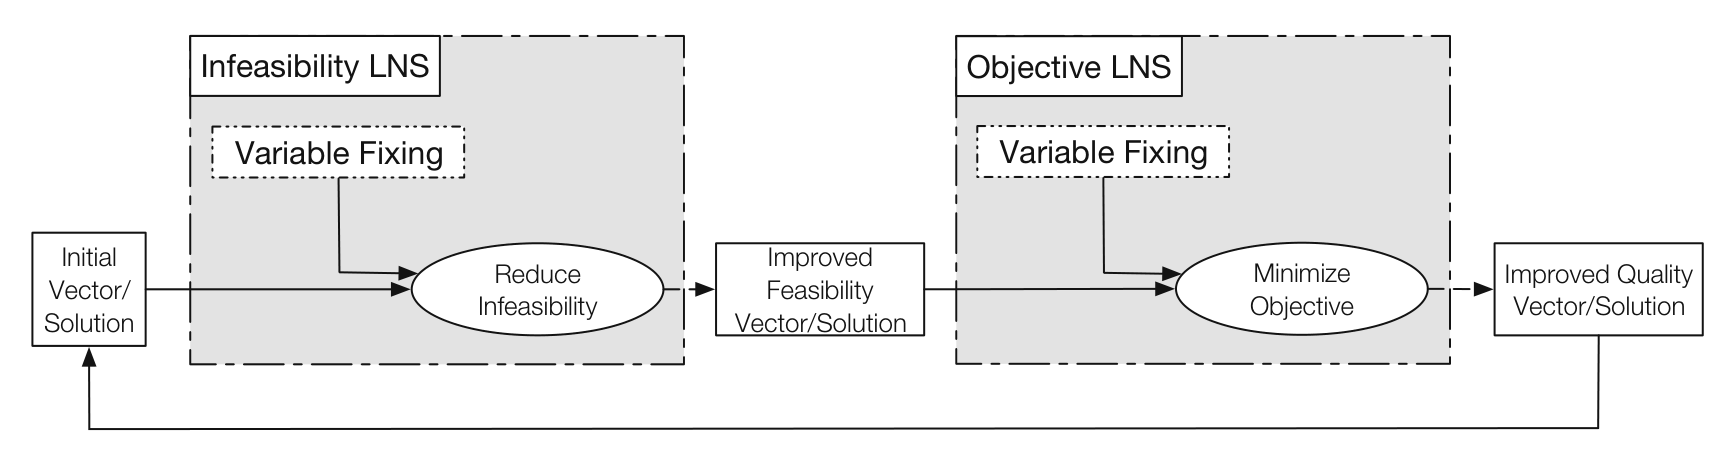
\includegraphics[scale=0.275]{img/diag_blocchi_acs}
\end{center}
\caption{Schema a blocchi del processo di esecuzione dell'algoritmo.}
\end{figure}

Per come sono costruiti i sub-MIP l'inammissibilità della soluzione decresce
in maniera monotona, tuttavia non è garantita la convergenza e per questo
motivo è necessario fissare dei limiti che consentano all'algoritmo di
terminare.
Questo ed altri parametri che verranno introdotti successivamente hanno 
un'influenza diretta sulle prestazioni dell'algoritmo.
La Figura~\ref{fig:andamento_objvfmip_objvomip} mostra il comportamento
ideale dell'algoritmo.

Una volta trovata una soluzione ammissibile, inizia una seconda fase in
cui viene risolto OMIP allo scopo di migliorare la qualità della soluzione.
Una volta conclusa anche questa fase, l'algoritmo termina restituendo la
soluzione trovata.

\begin{figure}[ht!]
\begin{center}
    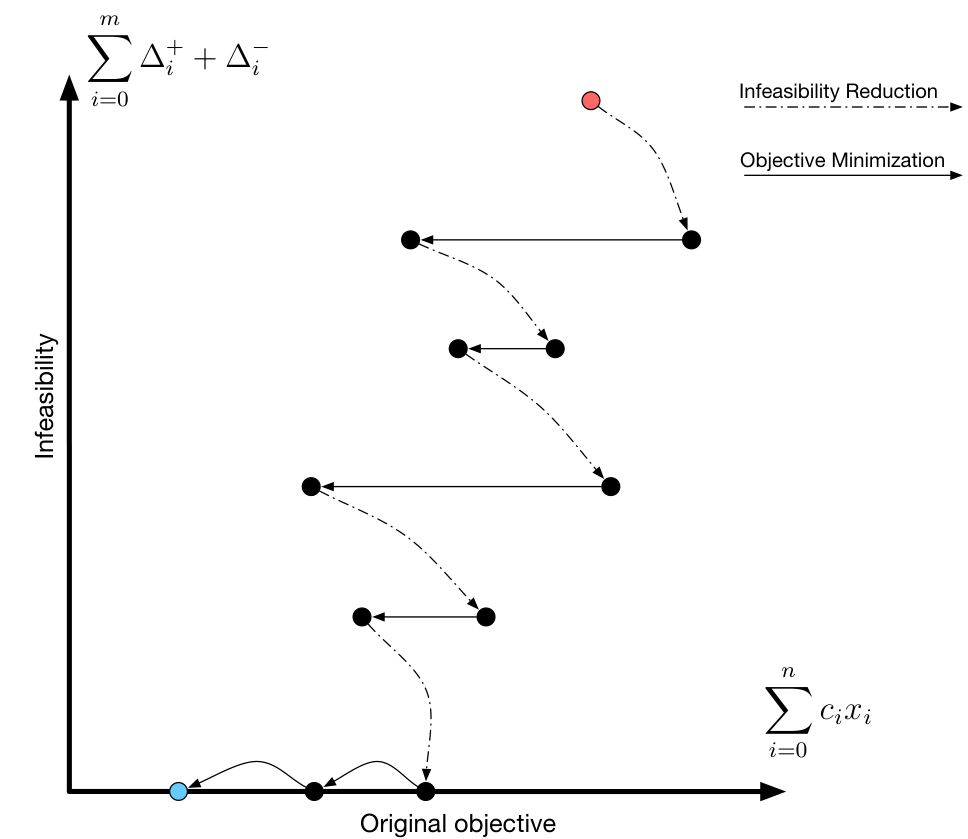
\includegraphics[scale=0.4]{img/andamento_objvfmip_objvomip.png}
\end{center}
\caption{Transizione da una soluzione non ammissibile (punto rosso) ad
una ammissibile qualitativamente buona (punto azzurro).}
\label{fig:andamento_objvfmip_objvomip}
\end{figure}

\begin{algorithm}
    \caption{Alternating Criteria Search} \label{alg:acs}
    \begin{algorithmic}
        \State $initialize \,\,[\hat x,\, \Delta^+,\, \Delta^-]$ \Comment Soluzione intera che rispetta i limiti
        \State $slack\_sum \gets -1$
        \For {$i\gets 1 \textbf{ to } MAX\_ITR$} \Comment MAX\_ITR va fissato
        \State $F \gets \text{randomized variable index subset, } F\subseteq I$
        \State $[\hat x,\, \Delta^+,\, \Delta^-] \gets \text{solve\_FMIP}(F,\,\hat x)$
        \State $slack\_sum\gets \sum_i \Delta^+_i + \Delta^-_i$
        \State $F \gets \text{randomized variable index subset, } F\subseteq I$
        \State $[\hat x,\, \Delta^+,\, \Delta^-] \gets \text{solve\_OMIP}(F,\,\hat x,\,sum\_slack)$
        \If {$\sum_i \Delta_i^+ + \Delta_i^- = 0$}
        \State break
        \EndIf
        \EndFor
        \State $z\gets 0$
        \Repeat \Comment Miglioramento qualità
        \State $z \gets c^t \hat x$
        \State $F \gets \text{randomized variable index subset, } F\subseteq I$
        \State $[\hat x,\, \Delta^+,\, \Delta^-] \gets \text{solve\_OMIP}(F,\,\hat x,\,0)$
        \Until {$c \hat x < z$}
        \State \Return $[\hat x,\, \Delta^+,\, \Delta^-]$
        \State
        \Function{solve\_FMIP}{$F,\, \hat x$}
        \State \Return $\min \{\sum_i \Delta_i^+ + \Delta_i^- | Ax + I_m\Delta^+ - I_m\Delta^- = b,\, x_j = \hat x_j\, \forall j\in F,\, x_j\in\Z\,\forall j\in I\}$
        \EndFunction
        \State
        \Function{solve\_OMIP}{$F,\, \hat x,\,\hat \Delta$}
        \State \Return $\min \{c^t x | Ax + I_m\Delta^+ - I_m\Delta^- = b,\, \sum_i \Delta_i^+ + \Delta_i^- \leq \hat \Delta,\,x_j = \hat x_j\, \forall j\in F,\, x_j\in\Z\,\forall j\in I\}$
        \EndFunction
    \end{algorithmic}
\end{algorithm}
